\documentclass{beamer}
\usepackage{tikz}
\usetikzlibrary{shapes,arrows}

\begin{document}

\begin{frame}{DNA Central Dogma}
    % Original TikZ code commented out - replaced with infographic image
    % \begin{tikzpicture}[node distance=3cm, auto]
    %     \tikzstyle{process} = [rectangle, minimum width=2cm, minimum height=1cm, text centered, draw=black, fill=blue!30]
    %     \tikzstyle{arrow} = [thick,->,>=stealth]
    %     \node (dna) [process] {DNA};
    %     \node (rna) [process, right of=dna] {RNA};
    %     \node (protein) [process, right of=rna] {Protein};
    %     \draw [arrow] (dna) -- node[anchor=south] {Transcription} (rna);
    %     \draw [arrow] (rna) -- node[anchor=south] {Translation} (protein);
    %     \draw [arrow] (dna) to [out=135,in=45,looseness=5] node[anchor=south] {Replication} (dna);
    % \end{tikzpicture}
    
    \centering
    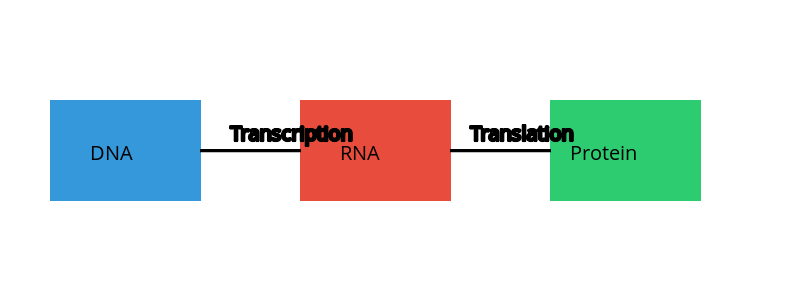
\includegraphics[width=0.9\textwidth, height=0.7\textheight, keepaspectratio]{images/central_dogma_infographic.png}
\end{frame}

\end{document}
